% 五号字体,开明式标点处理,不设置默认字体
\documentclass[UTF8,12pt,punct=kaiming,fontset=none]{ctexart}
\usepackage{fontspec}  % 字体
\usepackage{subcaption}  % 节标题
\usepackage[colorlinks=true, linkcolor=magenta, citecolor=magenta, urlcolor=magenta]{hyperref}  % 超链接
\usepackage{geometry}  % 页面布局
\usepackage{fancyhdr}  % 页眉页脚
\usepackage{titlesec}  % 标题
\usepackage{caption}  % 图表标题
\usepackage{floatrow}  % 图表排版
\usepackage{graphicx}  % 图片路径

% 图片路径
\graphicspath{{figures/}}

% 字体
\setCJKmainfont{Source Han Serif SC}
\setCJKsansfont{Source Han Sans SC}
\setmainfont{CMU Serif}

% 布局
\geometry{a4paper,left=2cm,right=2cm,top=2.5cm,bottom=2.5cm}
\setlength{\headheight}{25pt}

% 图表标题
\DeclareCaptionFont{captionfont}{\small}
\captionsetup{font=captionfont}
\floatsetup{style=plaintop}

% 页眉页脚
\pagenumbering{arabic}
\pagestyle{fancy}
\fancyhead[L]{· \hspace{0.1cm} \thepage \hspace{0.1cm} ·}
\fancyhead[C]{红 \hspace{0.08cm} 石 \hspace{0.08cm} 数 \hspace{0.08cm} 电 \hspace{0.08cm} 评 \hspace{0.08cm} 论\\\scriptsize{Review of Redstonic Digital Circuit}}
\fancyhead[R]{第1期\\\scriptsize{2022年2月}}
\fancyfoot[L,C,R]{}

% 首页页码
\input{页码.inc}

% 标题
\title{\vspace{-1.5cm}串行二进制转十进制方案\vspace{-0.5cm}}
\author{@天启c}
\date{}

% 参考文献标注
\newcommand*{\upcite}[1]{
    \textsuperscript{\cite{#1}}
}

\begin{document}
\pdfbookmark{串行二进制转十进制方案}{\thepage}  % 书签
\hypersetup{bookmarksdepth=-1}  % 禁止后续书签
\maketitle
\thispagestyle{fancy}  % 首页页眉页脚
\vspace{-0.7cm}

% 节标题格式
\titleformat{\section}[hang]{\large\sffamily\bfseries}{\textmd{\thesection}}{0.5cm}{}
\titlespacing{\section}{0cm}{0.5ex}{0.2ex}
\setcounter{section}{0}

数据在计算机中是二进制的形式存在的,十进制的数字同样也是用二进制数的形式存储。在计算机中通常有将十进制(BCD)码转换为二进制(BIN)码,又将二进制码转换为十进制码的操作。我们完全可以在Minecraft中将该操作进行还原。本文提出的“二转十”机器使用串行“满五加三”算法 \cite{5_3},以数据流移位器为核心,利用查表法执行算法,配合时钟和RS锁存器,可以每6tick计算一个二进制位。

串行信号首先发送到BIN码区,并不断向高位移位。超过8位的数据进入BCD码区。BCD码每四位一组依次代表十进制的某一位的值。在BIN码向BCD码移位操作过程中,我们通过“满五加三”算法完成由BIN码到BCD码的转换。这里我们通过查表法实现该算法。
    
\begin{figure}[!hb]
    \centering
    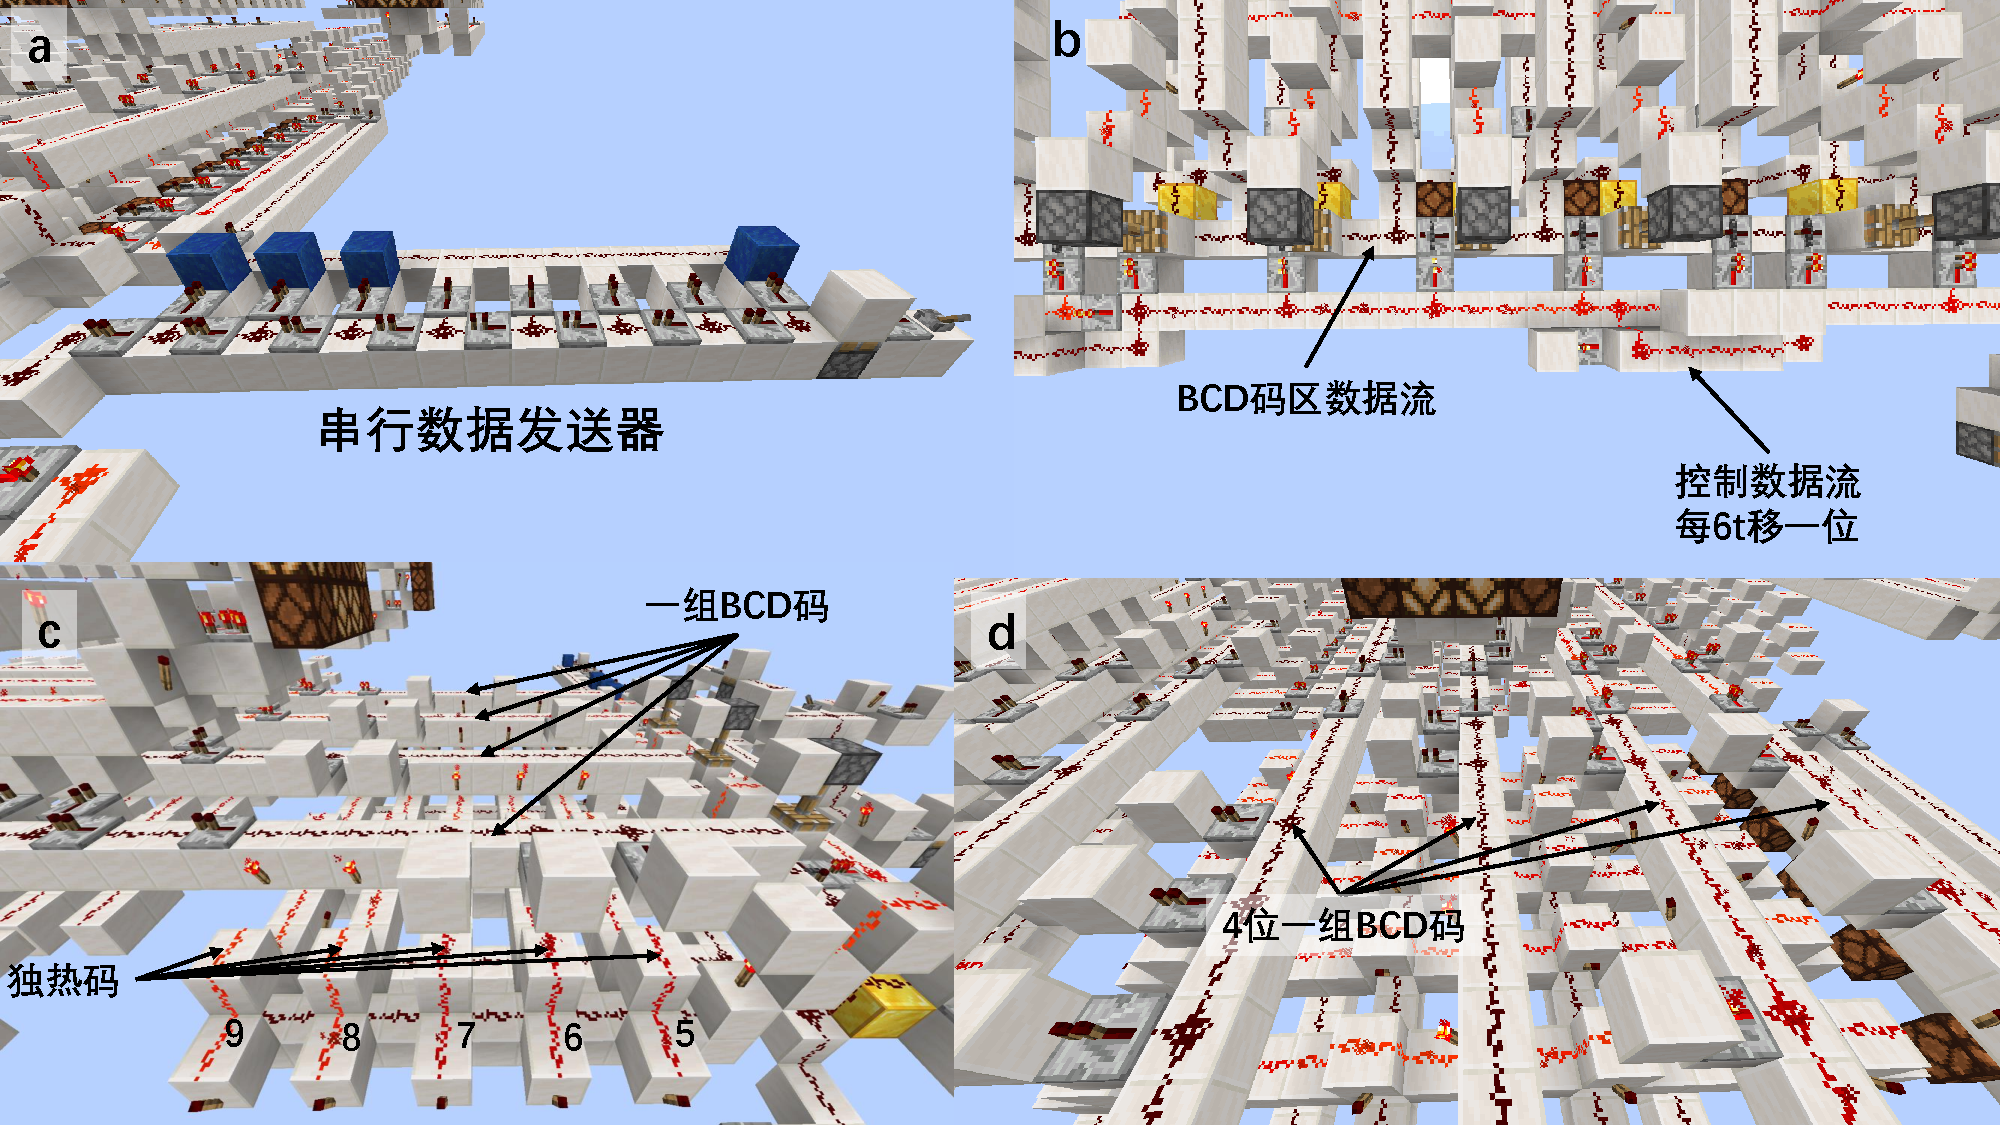
\includegraphics[width=.9\textwidth]{Fig_1.pdf}
    \caption{(a)(b) 串行数据发送器将数据流发送到移位器。(c)(d) 每一组BCD码信号按行输入,逐列比较。对于每一列独热码,红石火把代表1,红石中继器石英块代表0。当且仅当数值与某列信号匹配时,下方红石信号线(独热码线)熄灭,其上的红石火把点亮(独热码输出)。独热码会重新编码“加三”后的结果,并输出到(b)中金块的位置。}
    \label{fig:1}
\end{figure}

查表包含两个步骤。首先是寻址:将多个端口用二进制编码,并用二进制地址来激发相应端口。如果输入的是5,6,7,8,9(即满五),则寻址器会激发对应的独热码,见图\ref{fig:1}(c)(d)。接下来,被激发的独热码会通过解码器向数据流移位器反馈“加三”后的结果,即8,9,10,11,12,并替换该组BCD码。如果输入不满五,则不做动作。修改完毕后,BIN码和BCD码都向高位移动一位。重复这一流程直到BIN码区清空,则BCD码区就是输入转换成十进制的结果。

\begin{figure}[t]
    \centering
    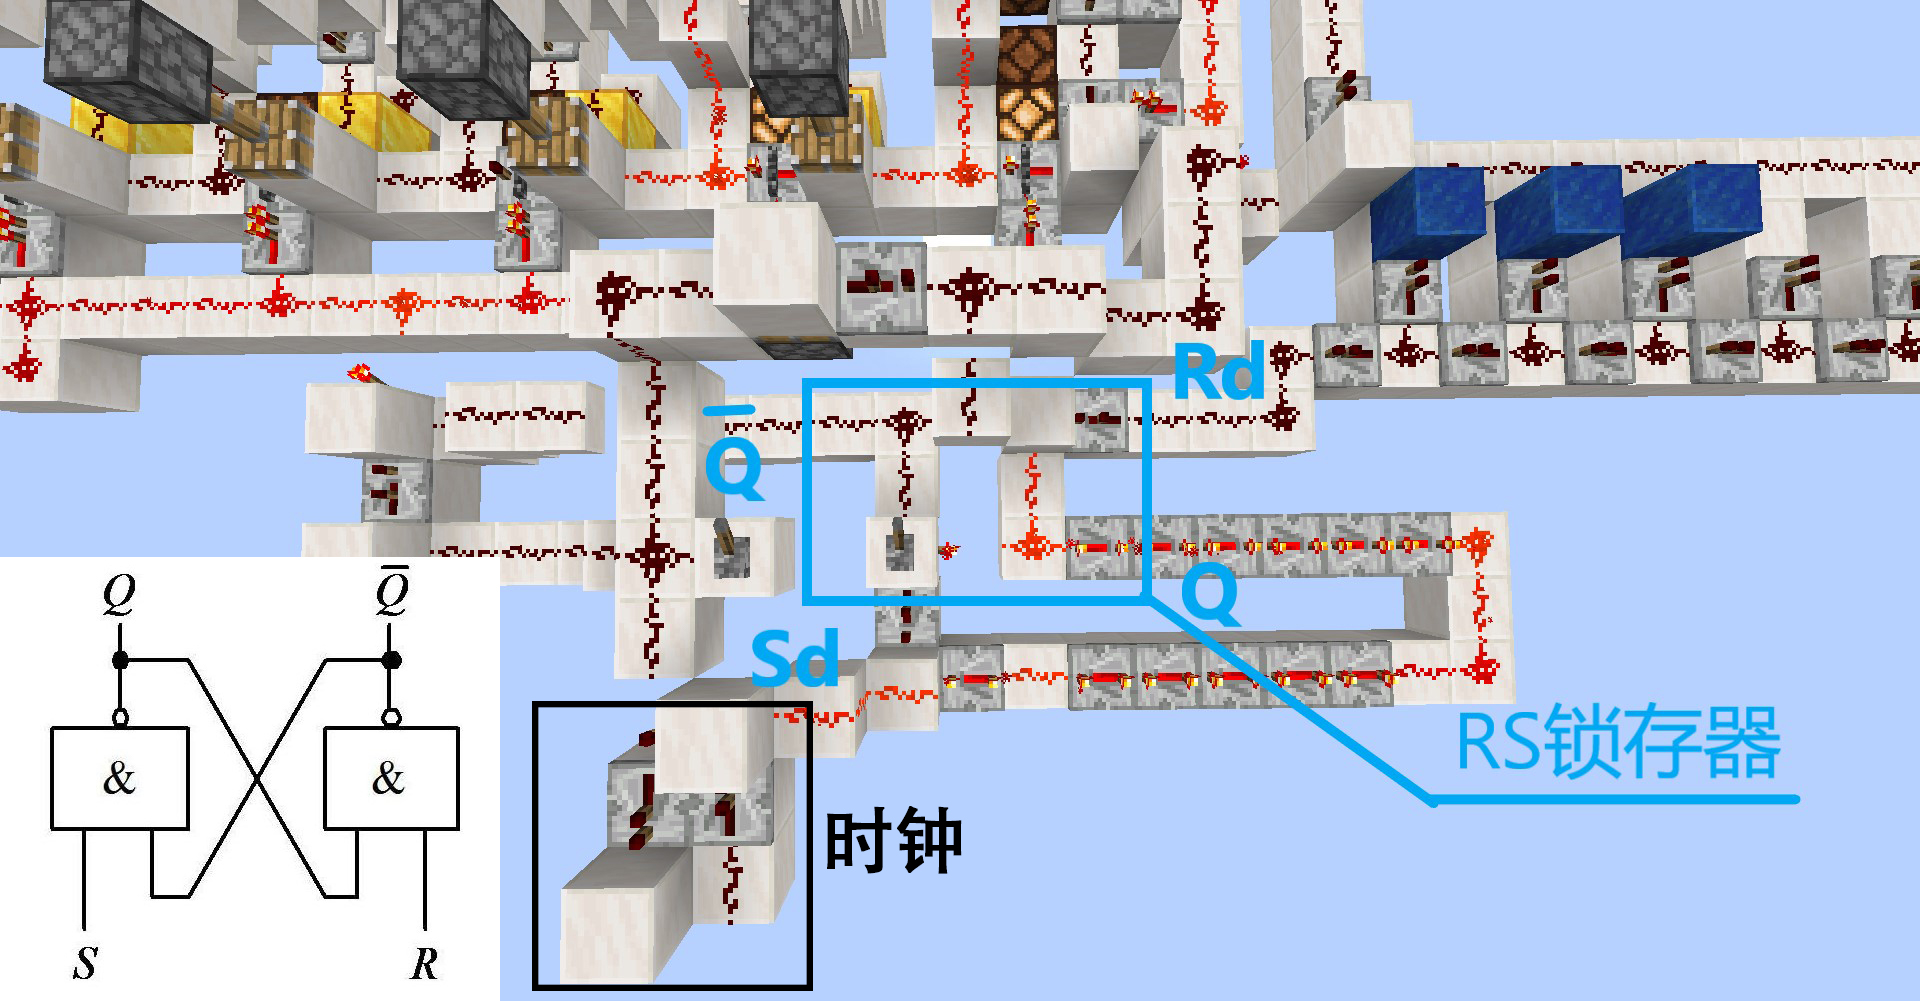
\includegraphics[width=.9\textwidth]{Fig_2.jpg}
    \caption{控制电路。开始信号以脉冲形式输入Rd并将RS锁存器置1,随后中继器链陆续熄灭,并在48tick后将RS锁存器清零。在RS锁存器置1期间,时钟启动并为机器提供6tick周期的脉冲信号。时钟输出的3tick脉冲会被调整为2tick,以此控制移位器每次移一位。左下角为RS锁存器逻辑电路。}
    \label{fig:2}
\end{figure}

控制组件包括一个周期为6tick的时钟,RS锁存器和一组48tick中继器延时,其目的是为机器提供8个时钟脉冲信号,见图\ref{fig:2}。不同的转换位数和布线方案会导致具体中继器延时与48tick有出入,需按具体情况作更改。

本文提出的串行“二转十”方案较并行方案体积小很多,而且很容易拓展,可以运用在四则计算器等需要显示十进制结果的机器上。为Minecraft数电红石技术发展新的计算器结构提供了新的研究方向。

\bibliographystyle{unsrt}
\bibliography{reference.bib}

\end{document}

